% Parameterized Fermion-to-Qubit Encodings — Algebraic Framework Paper
% Target: Quantum / Physical Review A / New Journal of Physics
% Compiled with: latexmk -pdf paper.tex
\documentclass[aps,pra,preprint,superscriptaddress,showpacs]{revtex4-2}

\usepackage[utf8]{inputenc}
\usepackage[T1]{fontenc}
\usepackage{lmodern}
\usepackage{amsmath,amssymb,amsfonts,amsthm}
\usepackage{booktabs}
\usepackage{hyperref}
\usepackage{graphicx}
\usepackage{xcolor}
\usepackage{tikz}
\usepackage{pgfplots}
\usepackage{braket}
\usepackage{mathtools}
\usepackage{cleveref}
\usepackage{siunitx}
\usepackage{algorithm}
\usepackage{algpseudocode}
\usepackage{array}
\usepackage{multirow}

\usetikzlibrary{trees,positioning,arrows.meta,calc}
\pgfplotsset{compat=1.18}

\hypersetup{
  colorlinks=true,
  linkcolor=blue!70!black,
  citecolor=green!50!black,
  urlcolor=blue!60!black,
}

% --- Custom commands ------------------------------------------------
\newcommand{\ad}[1]{a_{#1}^{\dagger}}       % creation operator
\newcommand{\an}[1]{a_{#1}^{\vphantom{\dagger}}} % annihilation operator
\newcommand{\nhat}[1]{\hat{n}_{#1}}          % number operator
\newcommand{\pauliw}[1]{w\!\left(#1\right)}  % Pauli weight
\newcommand{\acomm}[2]{\{#1,\,#2\}}         % anti-commutator
\newcommand{\comm}[2]{[#1,\,#2]}            % commutator
\newcommand{\Uset}[1]{U(#1)}                % update set
\newcommand{\Pset}[1]{P(#1)}                % parity set
\newcommand{\Rset}[1]{R(#1)}                % remainder set
\newcommand{\Occ}[1]{\mathrm{Occ}(#1)}      % occupation set
\newcommand{\depth}[1]{\mathrm{depth}(#1)}   % depth function
\newcommand{\CAR}{\mathrm{CAR}}
\newcommand{\CCR}{\mathrm{CCR}}
\newcommand{\encode}{\mathcal{E}}            % encoding map
\newcommand{\scheme}{\mathcal{S}}            % encoding scheme
\newcommand{\Qi}{\mathbb{Q}[i]}             % Gaussian rationals
\newcommand{\Zi}{\mathbb{Z}_4}              % cyclic group Z4

% Theorems
\newtheorem{theorem}{Theorem}
\newtheorem{corollary}[theorem]{Corollary}
\newtheorem{lemma}[theorem]{Lemma}
\newtheorem{proposition}[theorem]{Proposition}
\theoremstyle{definition}
\newtheorem{definition}[theorem]{Definition}
\theoremstyle{remark}
\newtheorem{remark}[theorem]{Remark}

%%====================================================================
\begin{document}

\title{Structural Limitations of Index-Set Fermion-to-Qubit Encodings}

\author{John Azariah}
\email{john.azariah@student.uts.edu.au}
\affiliation{University of Technology Sydney, Australia}

\date{\today}

%%--------------------------------------------------------------------
\begin{abstract}
The Seeley--Richard--Love (SRL) index-set framework is widely cited as
a unified treatment of fermion-to-qubit encodings, expressing
Jordan--Wigner, Bravyi--Kitaev, and Parity as instances of a single
parameterized map.  We prove that this unification is far less general
than commonly assumed: the generic index-set construction satisfies the
canonical anticommutation relations (CAR) \emph{if and only if} the
underlying tree is a star (depth~$\le 1$).  The proof identifies a
structural failure mode --- a parity-set cancellation along any
grandparent--parent--child path --- that is invisible when encodings
are studied individually.  The Bravyi--Kitaev encoding survives via a
separate Fenwick-specific construction, not the generic algorithm.  We
classify the space of $n^{n-1}$ labelled encoding trees into three
construction-compatibility regions and show that the path-based tree
construction is the only universal method.  We establish tight
Pauli-weight bounds determined by tree depth, with the balanced ternary
tree achieving optimal $O(\log_3 n)$ scaling.  All results are
validated by exact symbolic computation over 497 automated tests and
eigenspectrum comparison against molecular benchmarks.  An open-source
implementation accompanies this paper.
\end{abstract}

\maketitle

%%====================================================================
\section{Introduction}
\label{sec:intro}
% §1 Introduction — Restructured to lead with the star-tree theorem

Simulating fermionic systems on quantum hardware requires mapping the
anticommuting creation and annihilation operators of second quantization
to the tensor-product structure of qubit Pauli operators.  This
\emph{fermion-to-qubit encoding} directly determines the Pauli weight,
measurement complexity, and circuit depth of the resulting
simulation~\cite{tranter2015, havlicek2017}.

Five encodings dominate the literature: Jordan--Wigner~\cite{jordan1928},
Bravyi--Kitaev~\cite{bravyi2002, seeley2012}, Parity~\cite{seeley2012,
bravyi2017tapering}, balanced binary tree, and balanced ternary
tree~\cite{jiang2020, miller2023bonsai}.  Although each has been derived
independently, Seeley, Richard, and Love (SRL)~\cite{seeley2012}
observed that Jordan--Wigner, Bravyi--Kitaev, and Parity can all be
expressed via three set-valued functions --- update, parity, and
occupation sets --- applied to a universal encoding algorithm.  This
\emph{index-set framework} is widely cited as a unified treatment of
classical encodings and has been adopted as the standard explanation of
the Bravyi--Kitaev transform.

\subsection{The problem}

The SRL framework naturally suggests a generalization: given any rooted
tree on $n$ nodes, one can derive index sets by reading off ancestor,
child, and descendant relationships.  If valid, this would provide a
general-purpose encoding construction for arbitrary trees, not just the
Fenwick tree underlying Bravyi--Kitaev.

We show that this generalization fails.  The generic index-set
construction satisfies the canonical anticommutation relations (CAR)
\emph{if and only if} the tree is a star (depth $\le 1$).  This is a
far sharper restriction than previously recognized: out of $n^{n-1}$
labelled rooted trees on $n$ nodes, only $n$ are stars.

\subsection{Main result}

\begin{quotation}
\noindent\textbf{Star-tree theorem} (\cref{thm:star-tree}).
\emph{The index-set encoding construction, applied to a labelled
rooted tree~$T$, satisfies the CAR if and only if $T$ is a star
(every non-root vertex is a direct child of the root).}
\end{quotation}

The proof identifies a structural failure mode: on any path of length
$\geq 2$ (grandparent $w \to$ parent $u \to$ child $v$), the
symmetric-difference cancellation in the parity set assigns identity to
the middle node~$u$ in the Majorana operator $d_w$, while $c_v$ assigns
$X$ to all ancestors.  This produces exactly two anticommuting
positions (at $w$ and $v$), giving even parity --- the operators
commute instead of anticommute, violating the CAR.

\subsection{Consequences}

The star-tree theorem has several implications:

\begin{enumerate}
  \item \textbf{The SRL ``unification'' is narrower than assumed.}
    Jordan--Wigner and Parity correspond to star trees and are genuine
    instances of the generic construction.  But the Bravyi--Kitaev
    encoding uses a separate, Fenwick-specific construction
    (hand-derived bit-manipulation formulas) that is algebraically
    distinct from the generic algorithm applied to a Fenwick tree.  We
    call these Construction~A (generic index-set) and Construction~F
    (Fenwick-specific), respectively.

  \item \textbf{Three construction-compatibility regions.}  The space
    of $n^{n-1}$ encoding trees decomposes into: stars ($n$ trees,
    Construction~A valid), one Fenwick tree (Construction~F valid),
    and everything else (only the path-based Construction~B valid).

  \item \textbf{Path-based encoding is universal.}  The tree-path
    construction of Jiang et al.~\cite{jiang2020} and Miller et
    al.~\cite{miller2023bonsai}, which generates Pauli strings
    directly from root-to-leg paths, works for \emph{every} rooted
    tree.  It is the only universal encoding method.

  \item \textbf{Silent failures in the literature.}  Publications that
    apply ``the SRL method'' to arbitrary trees without independently
    verifying the CAR may contain encoding errors.  The failure mode
    is silent: the generic formula produces well-formed Pauli strings
    that appear correct but yield wrong eigenspectra.
\end{enumerate}

\subsection{Additional contributions}

Beyond the main theorem, this paper:
\begin{itemize}
  \item Establishes tight Pauli-weight bounds tied to tree depth:
    $w \le 2\,\depth{T} + 1$, with the balanced ternary tree achieving
    the optimal $O(\log_3 n)$ scaling (\cref{sec:constructions}).

  \item Shows that the count of index-monotonic labelled trees on $[n]$
    is $(n{-}1)!$, connecting encoding theory to heap-ordered tree
    enumeration (\cref{sec:star-tree}).

  \item Demonstrates that the encoding pipeline extends to bosonic
    commutation relations and mixed fermion--boson systems via an
    abstract combining algebra (\cref{sec:further}).

  \item Validates all results by exact symbolic computation: 497
    automated tests, eigenspectrum equivalence for H$_2$ (STO-3G),
    and exhaustive CAR verification for all trees at small~$n$
    (\cref{sec:validation}).
\end{itemize}

\subsection{Relation to prior work}

Seeley, Richard, and Love~\cite{seeley2012} introduced the update,
parity, and remainder sets for the Bravyi--Kitaev encoding and showed
that Jordan--Wigner and Parity can be expressed in the same language.
Their framework appeared to unify these three encodings under a single
index-set construction.  We show (\cref{sec:star-tree}) that this
unification covers only star trees, and the Bravyi--Kitaev encoding
uses a separate construction.

Steudtner and Wehner~\cite{steudtner2018} identified ternary tree
structure as a unifying construction and proved $O(\log_3 n)$ weight
bounds.  Jiang et al.~\cite{jiang2020} gave the path-based
construction, and Miller et al.~\cite{miller2023bonsai} generalized to
arbitrary tree topologies.  Our star-tree theorem provides a
retroactive explanation of why the path-based construction was
necessary: the index-set alternative fails for all but the simplest
trees.

\subsection{Outline}

\Cref{sec:prelim} establishes notation and reviews the Majorana
decomposition.  \Cref{sec:constructions} defines the two encoding
constructions (index-set and path-based) side by side.
\Cref{sec:star-tree} presents the star-tree theorem with its
structural proof, failure-mode analysis, and encoding-space
classification.  \Cref{sec:validation} gives computational validation.
\Cref{sec:further} summarizes additional results on algebraic
exactness and bosonic extensions.  \Cref{sec:discussion} discusses
implications and open questions.


%%====================================================================
\section{Preliminaries}
\label{sec:prelim}
% §2 Preliminaries

We establish the notation, collect the key definitions used throughout,
and review the standard Majorana decomposition that underpins both
parameterized maps.

\subsection{Fermionic operators and canonical anticommutation relations}

Consider $n$ fermionic modes with creation operators $\ad{j}$ and
annihilation operators $\an{j}$ for $j \in \{0, \ldots, n{-}1\}$.
These satisfy the \emph{canonical anticommutation relations} (CAR):
\begin{align}
  \acomm{\an{i}}{\ad{j}} &= \delta_{ij}, \label{eq:car1} \\
  \acomm{\an{i}}{\an{j}} &= 0, \label{eq:car2} \\
  \acomm{\ad{i}}{\ad{j}} &= 0. \label{eq:car3}
\end{align}
These relations ensure the Pauli exclusion principle: no two fermions
can occupy the same mode.

\subsection{Pauli algebra}

A qubit register of $n$ qubits admits the Pauli group $\mathcal{P}_n$
consisting of $n$-fold tensor products of single-qubit Pauli operators
$\{I, X, Y, Z\}$ with phases in $\{+1, -1, +i, -i\}$.  The
single-qubit multiplication table is:
\begin{equation}
  XY = iZ, \quad YZ = iX, \quad ZX = iY,
  \label{eq:pauli-products}
\end{equation}
with $\sigma^2 = I$ for all $\sigma \in \{X, Y, Z\}$ and
$\sigma_a \sigma_b = -\sigma_b \sigma_a$ for $a \neq b$.
Multi-qubit Pauli strings multiply componentwise:
\begin{equation}
  (\sigma_{a_0} \otimes \cdots \otimes \sigma_{a_{n-1}})
  (\sigma_{b_0} \otimes \cdots \otimes \sigma_{b_{n-1}})
  = \phi \cdot
  (\sigma_{a_0}\sigma_{b_0}) \otimes \cdots \otimes
  (\sigma_{a_{n-1}}\sigma_{b_{n-1}}),
  \label{eq:pauli-mult}
\end{equation}
where $\phi = \prod_{k=0}^{n-1} \phi_k$ is the accumulated phase from
each single-qubit multiplication.  The \emph{Pauli weight} of a string
is the number of non-identity factors.

\subsection{Core definitions}
\label{sec:core-defs}

We collect the central definitions used throughout the paper.  Further
definitions (index-monotonic trees, star trees) are introduced in
\cref{sec:star-tree} where they are needed for the main theorem.

\begin{definition}[Phase group]
\label{def:phase-group}
The \emph{phase group} $\Zi = \{+1, -1, +i, -i\}$ is the cyclic group
of order~4 under multiplication.  We write elements as $\{P_1, M_1,
P_i, M_i\}$.  Every single-qubit Pauli product yields a result Pauli
and a phase element in $\Zi$.
\end{definition}

\begin{definition}[Majorana operators]
\label{def:majorana}
For each mode $j$, the Hermitian \emph{Majorana operators} are:
\begin{align}
  c_j &= \ad{j} + \an{j}, \label{eq:majorana-c} \\
  d_j &= i(\ad{j} - \an{j}). \label{eq:majorana-d}
\end{align}
These satisfy $\{c_i, c_j\} = 2\delta_{ij}$,
$\{d_i, d_j\} = 2\delta_{ij}$, and $\{c_i, d_j\} = 0$.
\end{definition}

\noindent
Inverting~\eqref{eq:majorana-c}--\eqref{eq:majorana-d}:
\begin{equation}
  \ad{j} = \tfrac{1}{2}(c_j - id_j), \qquad
  \an{j} = \tfrac{1}{2}(c_j + id_j).
  \label{eq:ladder-from-majorana}
\end{equation}

\begin{definition}[Fermion-to-qubit encoding]
\label{def:encoding}
A \emph{fermion-to-qubit encoding} for $n$ modes on $n$ qubits is a
pair of maps $c_j \mapsto S_j^{(c)}$ and $d_j \mapsto S_j^{(d)}$, where
each $S_j^{(c)}$ and $S_j^{(d)}$ is a Pauli string (an element of
$\mathcal{P}_n$), such that the induced ladder operators
\begin{equation}
  \ad{j} = \tfrac{1}{2}(S_j^{(c)} - i S_j^{(d)}), \qquad
  \an{j} = \tfrac{1}{2}(S_j^{(c)} + i S_j^{(d)})
  \label{eq:encoded-ladder}
\end{equation}
satisfy the CAR~\eqref{eq:car1}--\eqref{eq:car3}.
\end{definition}

\begin{definition}[Encoding scheme]
\label{def:encoding-scheme}
An \emph{encoding scheme} is a triple of set-valued functions
$\scheme = (\Uset{\cdot}, \Pset{\cdot}, \Occ{\cdot})$ from mode
indices $\{0, \ldots, n{-}1\}$ to subsets of qubit indices
$\{0, \ldots, n{-}1\}$, from which Majorana operators can be
constructed via a universal algorithm (\cref{sec:constructions}).
\end{definition}

\begin{definition}[Combining algebra]
\label{def:combining-algebra}
A \emph{combining algebra} is a function that specifies how to
reorder a ladder operator past another during normal ordering.  The
two instances are:
\begin{itemize}
  \item \emph{Fermionic} (CAR): swapping $\an{j}$ past $\ad{k}$
    with $j = k$ produces two terms with a sign flip
    ($\an{j}\ad{j} = \delta_{jj} - \ad{j}\an{j}$).
  \item \emph{Bosonic} (CCR): swapping $b_j$ past $b_k^\dagger$
    with $j = k$ produces two terms with no sign change
    ($b_j b_j^\dagger = b_j^\dagger b_j + 1$).
\end{itemize}
\end{definition}

\noindent
The central observation is that every known encoding can be specified
by describing how to construct $S_j^{(c)}$ and $S_j^{(d)}$, and two
distinct parameterizations accomplish this.

\subsection{The electronic Hamiltonian}

The second-quantized electronic Hamiltonian is:
\begin{equation}
  H = \sum_{pq} h_{pq}\, \ad{p}\an{q}
    + \frac{1}{2} \sum_{pqrs} g_{pqrs}\, \ad{p}\ad{q}\an{s}\an{r},
  \label{eq:hamiltonian}
\end{equation}
where $h_{pq}$ are one-electron integrals and $g_{pqrs}$ are
two-electron integrals from quantum chemistry
computations~\cite{szabo1996, helgaker2000}.  An encoding maps each
$\ad{j}$ and $\an{j}$ to a two-term Pauli expression
via~\eqref{eq:encoded-ladder}, and the products are expanded using the
Pauli multiplication rule~\eqref{eq:pauli-mult}.  The result is a
Hamiltonian expressed entirely in terms of Pauli strings:
\begin{equation}
  H = \sum_{\alpha} h_\alpha\, \sigma_\alpha,
  \label{eq:pauli-hamiltonian}
\end{equation}
where $\sigma_\alpha \in \mathcal{P}_n$ and $h_\alpha \in \mathbb{C}$.


%%====================================================================
\section{Two Encoding Constructions}
\label{sec:constructions}
% §3 Two Encoding Constructions
%
% Merges old §3 (index-set) and §4 (tree-encoding) into a single
% side-by-side presentation.  Fixes the formula inconsistency between
% eq (7) (SRL) and the code/proof formula.

We now define the two parameterized maps that generate fermion-to-qubit
encodings.  Both factor through the Majorana intermediate representation
(\cref{def:majorana}), separating encoding \emph{definition} from
encoding \emph{computation}.

%%====================================================================
\subsection{Construction~A: Index-set schemes}
\label{sec:index-set}

\begin{definition}[Index-set scheme]
\label{def:index-set-scheme}
An \emph{index-set encoding scheme} for $n$ modes is a triple of
set-valued functions $\scheme = (U, P, \mathrm{Occ})$:
\begin{align}
  U &: \{0, \ldots, n{-}1\} \to 2^{\{0,\ldots,n{-}1\}},
    \label{eq:update-fn} \\
  P &: \{0, \ldots, n{-}1\} \to 2^{\{0,\ldots,n{-}1\}},
    \label{eq:parity-fn} \\
  \mathrm{Occ} &: \{0, \ldots, n{-}1\} \to 2^{\{0,\ldots,n{-}1\}}.
    \label{eq:occ-fn}
\end{align}
We call $U(j)$ the \emph{update set}, $P(j)$ the \emph{parity set},
and $\mathrm{Occ}(j)$ the \emph{occupation set} of mode~$j$.
\end{definition}

\paragraph{The encoding algorithm.}
Given a scheme~$\scheme$, the Majorana operators for mode~$j$ are:
\begin{align}
  c_j &= X_{\{j\} \cup U(j)} \;\cdot\; Z_{P(j)},
  \label{eq:cj-from-scheme} \\[4pt]
  d_j &= Y_j \;\cdot\; X_{U(j)} \;\cdot\;
    Z_{(P(j)\,\triangle\,\mathrm{Occ}(j))\,\setminus\,\{j\}},
  \label{eq:dj-from-scheme}
\end{align}
where $X_S$ denotes $X$ on every qubit in set~$S$ (identity elsewhere),
$\triangle$ is the symmetric difference, and qubit positions in
multiple sets are resolved left-to-right (the first assignment
wins).  The sets $\{j\} \cup U(j)$ and $P(j)$ are required to be
disjoint for the formula to be unambiguous; we verify this as part of
the correctness check.

The ladder operators are then given by~\eqref{eq:encoded-ladder}.

\begin{remark}[Relation to the SRL formula]
\label{rem:srl}
Seeley, Richard, and Love~\cite{seeley2012} present a more complex
formula that places $Y$ at positions in $\mathrm{Occ}(j) \cap P(j)$
and $X$ at $\mathrm{Occ}(j) \setminus P(j)$.  For the three classical
schemes (JW, BK, Parity), the sets $\{j\} \cup U(j)$ and $P(j)$ are
disjoint, and both formulas produce identical Majorana operators.  Our
simpler formulation~\eqref{eq:cj-from-scheme}--\eqref{eq:dj-from-scheme}
suffices for the structural analysis of \cref{sec:star-tree} and
matches the implementation.
\end{remark}

\paragraph{Three classical encodings as set triples.}
\begin{align}
  \text{JW:}\;&\;
    U(j) = \emptyset,\;
    P(j) = \{0,\ldots,j{-}1\},\;
    \mathrm{Occ}(j) = \{j\}.
    \label{eq:jw-scheme} \\[3pt]
  \text{Parity:}\;&\;
    U(j) = \{j{+}1,\ldots,n{-}1\},\;
    P(j) = \{j{-}1\}^*,\;
    \mathrm{Occ}(j) = \{j{-}1,j\}^*.
    \label{eq:parity-scheme} \\[3pt]
  \text{BK:}\;&\;
    U, P, \mathrm{Occ}\text{ from the Fenwick tree}
    ~\cite{fenwick1994, seeley2012}.
    \label{eq:bk-scheme}
\end{align}
(Starred entries: for $j = 0$, $P(0) = \emptyset$ and
$\mathrm{Occ}(0) = \{0\}$.)

All variation between encodings is captured in the three
functions.  The encoding algorithm itself never changes.

\paragraph{Deriving index sets from a tree.}
Given a labelled rooted tree $T$ on $[n]$, one can attempt to derive
a scheme by reading off structural relationships:
\begin{align}
  U(j) &= \text{ancestors of } j, \notag \\
  P(j) &= \text{remainder}(j) \cup \text{children}(j), \notag \\
  \mathrm{Occ}(j) &= \text{descendants}(j) \cup \{j\},
  \label{eq:tree-derived-sets}
\end{align}
where $\text{remainder}(j)$ collects children of ancestors of $j$
that have index $< j$ and are not themselves ancestors of~$j$.

This derivation always produces well-formed sets and yields Pauli
strings of the correct width.  The question is whether the resulting
encoding satisfies the CAR.  We prove in \cref{sec:star-tree} that it
does \emph{if and only if} the tree is a star.

%%====================================================================
\subsection{Construction~B: Path-based tree encodings}
\label{sec:tree-encoding}

\begin{definition}[Encoding tree]
\label{def:encoding-tree}
An \emph{encoding tree} for $n$ fermionic modes is a rooted tree $T$
with internal nodes, where each node has at most three descending
connections, each labelled by a distinct Pauli operator from $\{X, Y,
Z\}$.  Each connection is either an \emph{edge} (to a child node) or a
\emph{leg} (a dangling link).  The total number of legs is $2n$, paired
into $n$ mode assignments.
\end{definition}

\paragraph{The encoding algorithm.}
For mode~$j$, let $\ell_j^{(x)}$ and $\ell_j^{(y)}$ be the paired
legs.  The Majorana operator for each leg is the Pauli string obtained
by collecting the link labels along the root-to-leg path:
\begin{equation}
  S(\ell) = \bigotimes_{v \in \mathrm{path}(\ell)}
    \text{label}(v \to \text{next}) \;\otimes\;
    \bigotimes_{v \notin \mathrm{path}(\ell)} I.
  \label{eq:path-pauli}
\end{equation}
The ladder operators are:
$\ad{j} = \tfrac{1}{2}(S(\ell_j^{(x)}) - i\,S(\ell_j^{(y)}))$.

\begin{theorem}[Tree encoding correctness]
\label{thm:tree-car}
For any encoding tree $T$ with $2n$ legs paired into $n$ modes, the
ladder operators satisfy the CAR.
\end{theorem}

\begin{proof}[Proof sketch]
Legs on distinct subtrees produce Pauli strings with disjoint
non-identity support except at the branching ancestor, where distinct
labels ($X$, $Y$, $Z$) ensure anticommutation.  Legs sharing a prefix
differ in the subtree below the branch point.  The proof follows Jiang
et al.~\cite{jiang2020} by induction on tree depth.
\end{proof}

\paragraph{Recovery of known encodings.}
All five standard encodings arise from specific tree topologies:
\begin{center}
\begin{tabular}{@{}lll@{}}
\toprule
Tree topology & Encoding & Max Pauli weight \\
\midrule
Star (depth 1, chain ordering) & Jordan--Wigner & $O(n)$ \\
Star (depth 1, reversed) & Parity & $O(n)$ \\
Fenwick tree & Bravyi--Kitaev & $O(\log_2 n)$ \\
Balanced binary tree & Binary tree & $O(\log_2 n)$ \\
Balanced ternary tree & Ternary tree & $O(\log_3 n)$ \\
\bottomrule
\end{tabular}
\end{center}

%%====================================================================
\subsection{Pauli-weight bounds}
\label{sec:weight-bounds}

\begin{theorem}[Weight bound]
\label{thm:weight-bound}
For an encoding tree $T$ with depth $d = \depth{T}$, every encoded
ladder operator has Pauli weight at most $2d + 1$.
\end{theorem}

\begin{proof}
Each Majorana string has weight equal to the root-to-leg path length,
at most $d + 1$.  The worst-case ladder operator (sum of two Majorana
strings sharing only the root) has weight at most $2d + 1$.
\end{proof}

\begin{corollary}[Optimal asymptotic weight]
\label{cor:optimal-weight}
Since each node has at most 3 children (one per Pauli label), the
balanced ternary tree achieves optimal weight $O(\log_3 n)$ among
fixed-arity trees.
\end{corollary}

%%====================================================================
\subsection{Three constructions, not two}
\label{sec:three-constructions}

A key observation is that the literature contains three distinct
encoding constructions, each with a different domain of validity:

\begin{description}
  \item[Construction~A] (index-set method,
    \cref{sec:index-set}): derives index sets from a tree via
    \eqref{eq:tree-derived-sets} and applies the universal
    algorithm~\eqref{eq:cj-from-scheme}--\eqref{eq:dj-from-scheme}.
    Valid only for star trees (\cref{sec:star-tree}).

  \item[Construction~B] (path-based method,
    \cref{sec:tree-encoding}): generates Pauli strings directly from
    root-to-leg paths.  Universal: valid for every encoding tree.

  \item[Construction~F] (Fenwick-specific): the Bravyi--Kitaev
    encoding uses hand-derived bit-manipulation formulas for $U$, $P$,
    $\mathrm{Occ}$ that exploit the unique algebraic structure of the
    Fenwick tree~\cite{fenwick1994}.  These formulas produce a correct
    encoding but are not the same as the generic tree-derived sets of
    Construction~A applied to a Fenwick-shaped tree.
\end{description}

The SRL ``unification'' of JW, BK, and Parity into a single index-set
framework is, on inspection, a conflation of Constructions~A and~F.
JW and Parity are genuine Construction~A instances (star trees).  BK
is a Construction~F instance that happens to be \emph{expressible} as
an index-set scheme, but the scheme is hand-derived for the Fenwick
tree rather than mechanically extracted.


%%====================================================================
\section{The Star-Tree Theorem}
\label{sec:star-tree}
% §4 The Star-Tree Theorem
%
% Restructured from old §5: leads with structural proof, enumeration
% as independent validation.  This is the heart of the paper.

We now prove the main result: Construction~A satisfies the CAR if and
only if the tree is a star.

%%====================================================================
\subsection{Definitions}
\label{sec:st-definitions}

\begin{definition}[Star tree]
\label{def:star}
A labelled rooted tree $T$ on $[n]$ is a \emph{star} if every
non-root vertex is a direct child of the root, i.e., $T$ has
depth~$\le 1$.
\end{definition}

\begin{definition}[Index-monotonic tree]
\label{def:monotonic}
A labelled rooted tree $T$ on $[n]$ is \emph{index-monotonic} if for
every vertex $v$ and every ancestor $u$ of $v$,
$\mathrm{label}(u) > \mathrm{label}(v)$.  Equivalently, labels
strictly decrease on every root-to-leaf path.
\end{definition}

Every star is monotonic (depth~1 paths are trivially decreasing), but
most monotonic trees are not stars.  Monotonicity is neither necessary
nor sufficient for Construction~A correctness; the star condition is
both necessary and sufficient.

%%====================================================================
\subsection{Statement and proof}
\label{sec:st-proof}

\begin{theorem}[Star-tree constraint]
\label{thm:star-tree}
Let $T$ be a labelled rooted tree on $[n]$, and let $(U, P,
\mathrm{Occ})$ be the tree-derived index-set
scheme~\eqref{eq:tree-derived-sets}.  The Majorana operators defined
by~\eqref{eq:cj-from-scheme}--\eqref{eq:dj-from-scheme} satisfy the
CAR if and only if $T$ is a star.
\end{theorem}

\begin{proof}[Proof of sufficiency]
Let $T$ be a star with root~$r$ and leaves $L = \{l_1, \ldots,
l_{n-1}\}$.  For any leaf~$j$:
\[
  U(j) = \{r\}, \quad
  P(j) = \{k \in L : k < j\}, \quad
  \mathrm{Occ}(j) = \{j\}.
\]
Since $U(j) \cap P(j) = \emptyset$ and $\{j\} \cap P(j) = \emptyset$,
the formula~\eqref{eq:cj-from-scheme} is unambiguous.  We verify the
Majorana anticommutation relations directly.

\emph{Case 1: distinct leaves $j < k$.}
$c_j$ has $X_j X_r Z_{\{<j\}}$ and $c_k$ has $X_k X_r Z_{\{<k\}}$.
At position~$r$: $X \cdot X$ commutes.  At position~$j$: $c_j$ has
$X$, $c_k$ has $Z$ (since $j < k$ implies $j \in P(k)$);
anticommutes.  No other position has non-identity in both.  Total
anticommuting positions: 1 (odd).  So $\{c_j, c_k\} = 0$.

\emph{Case 2: root $r$ and leaf $j$.}
$c_r$ has $X_r Z_L$ and $c_j$ has $X_j X_r Z_{\{<j\}}$.
At~$r$: $X \cdot X$ commutes.  At~$j$: $c_r$ has $Z$ (since
$j \in L \subset P(r)$), $c_j$ has $X$; anticommutes.  Total: 1
(odd).  So $\{c_r, c_j\} = 0$.

The $d$--$d$ and $c$--$d$ relations follow analogously, using the
symmetric-difference formula~\eqref{eq:dj-from-scheme}.  In every
case, exactly one position anticommutes, giving odd total parity.
\end{proof}

\begin{proof}[Proof of necessity]
Suppose $T$ is \emph{not} a star.  Then $T$ has depth~$\ge 2$, and
there exists a path $w \to u \to v$ of length two, where $w$ is the
grandparent, $u$ is the parent, and $v$ is the grandchild.

We show that $\{d_w, c_v\} \neq 0$, violating the Majorana CAR
requirement $\{c_i, d_j\} = 0$ for all $i, j$.

\textbf{Step 1: Identify the Pauli assignments.}
From~\eqref{eq:cj-from-scheme}, the operator $c_v$ has:
\begin{equation}
  c_v = X_{\{v\} \cup U(v)} \;\cdot\; Z_{P(v)}.
  \label{eq:cv-explicit}
\end{equation}
Since $w$ and $u$ are both ancestors of $v$, position $w$ and position
$u$ both receive $X$.

From~\eqref{eq:dj-from-scheme}, the operator $d_w$ has:
\begin{equation}
  d_w = Y_w \;\cdot\; X_{U(w)} \;\cdot\;
    Z_{(P(w)\,\triangle\,\mathrm{Occ}(w))\,\setminus\,\{w\}}.
  \label{eq:dw-explicit}
\end{equation}

\textbf{Step 2: Determine $d_w$ at position $u$.}
Node $u$ is a child of $w$, so $u \in \text{children}(w) \subseteq
P(w)$.  Node $u$ is also a descendant of $w$, so $u \in \mathrm{Occ}(w)$.
Therefore $u \in P(w) \cap \mathrm{Occ}(w)$, which means $u$ cancels in
the symmetric difference $P(w) \triangle \mathrm{Occ}(w)$.  Since $u$ is
not an ancestor of $w$, $u \notin U(w)$.  Hence:
\[
  d_w \text{ at position } u = I \quad\text{(identity)}.
\]

\textbf{Step 3: Determine $d_w$ at position $v$.}
Node $v$ is a descendant of $w$ (grandchild), so
$v \in \mathrm{Occ}(w)$.  But $v$ is \emph{not} a child of $w$ (it is
a grandchild), and $v$ is not in $\text{remainder}(w)$ because
$\text{remainder}(w)$ collects children of ancestors of $w$, which are
nodes \emph{above} $w$ in the tree, not below.  Therefore
$v \notin P(w)$, whence $v \in \mathrm{Occ}(w) \setminus P(w) \subset
P(w) \triangle \mathrm{Occ}(w)$.  Hence:
\[
  d_w \text{ at position } v = Z.
\]

\textbf{Step 4: Count anticommuting positions.}
\begin{center}
\begin{tabular}{@{}ccccl@{}}
\toprule
Position & $d_w$ & $c_v$ & Anticommute? & Reason \\
\midrule
$w$ & $Y$ & $X$ & Yes & $w \in U(v)$, first term of $d_w$ \\
$u$ & $I$ & $X$ & No  & $u$ cancelled (Step~2) \\
$v$ & $Z$ & $X$ & Yes & $v \in \mathrm{Occ} \setminus P$ (Step~3) \\
\bottomrule
\end{tabular}
\end{center}
At positions above $w$ (ancestors of $w$): both $d_w$ and $c_v$ have
the same Pauli ($X$ from their respective update sets), so they
commute.  At all other positions (siblings, cousins, deeper
descendants not on the path), at least one operator has identity.  The
total count of anticommuting positions is $1 + 0 + 1 = 2$ (even).

Therefore $d_w c_v = +c_v d_w$, whence $\{d_w, c_v\} = 2\,d_w c_v
\neq 0$, violating the CAR.  Since every non-star tree has
depth~$\ge 2$ and thus contains such a path, only stars are valid.
\end{proof}

\begin{figure}[t]
\centering
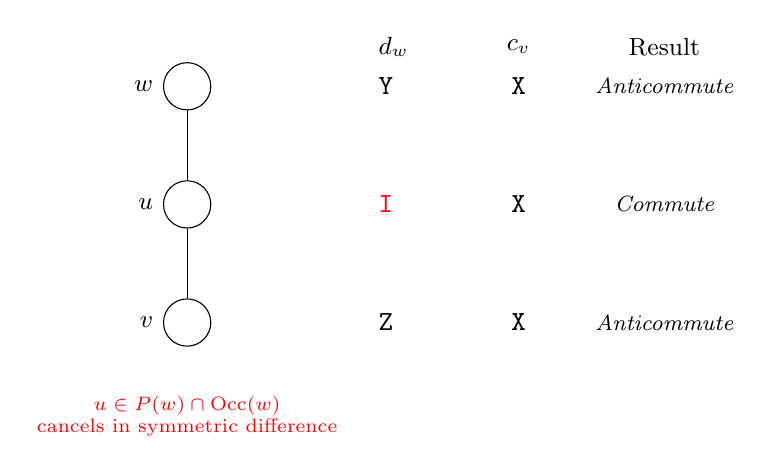
\begin{tikzpicture}[
  node distance=1.5cm,
  every node/.style={font=\small},
  treeNode/.style={circle, draw, minimum size=0.6cm, inner sep=0pt},
  pauli/.style={font=\ttfamily\bfseries},
  comm/.style={font=\footnotesize\itshape}
]
  % Tree structure
  \node[treeNode, label=left:$w$] (w) {};
  \node[treeNode, label=left:$u$, below of=w] (u) {};
  \node[treeNode, label=left:$v$, below of=u] (v) {};
  \draw (w) -- (u) -- (v);

  % Column headers
  \node[right=2cm of w, yshift=0.5cm] (h1) {$d_w$};
  \node[right=1cm of h1] (h2) {$c_v$};
  \node[right=1cm of h2] (h3) {Result};

  % Row w
  \node[pauli, right=2cm of w] (dw_w) {Y};
  \node[pauli] at (dw_w -| h2) (cv_w) {X};
  \node[comm]  at (dw_w -| h3) {Anticommute};

  % Row u
  \node[pauli, right=2cm of u, color=red] (dw_u) {I};
  \node[pauli] at (dw_u -| h2) (cv_u) {X};
  \node[comm]  at (dw_u -| h3) {Commute};

  % Row v
  \node[pauli, right=2cm of v] (dw_v) {Z};
  \node[pauli] at (dw_v -| h2) (cv_v) {X};
  \node[comm]  at (dw_v -| h3) {Anticommute};

  % Annotation
  \node[below=0.5cm of v, font=\scriptsize, color=red, align=center]
    {$u \in P(w) \cap \mathrm{Occ}(w)$\\cancels in symmetric difference};
\end{tikzpicture}
\caption{The structural failure mode.  On any depth-$\ge 2$ path
$w \to u \to v$, the symmetric-difference cancellation assigns
identity to $u$ in $d_w$ (red), while $c_v$ assigns $X$ to all
ancestors.  The even count of anticommuting positions (2) causes the
operators to commute instead of anticommute.}
\label{fig:structural-failure}
\end{figure}

\paragraph{Remark.}
The proof does not depend on the tree labelling: the failure arises
from the tree \emph{shape} (having depth~$\ge 2$), not the specific
index assignments.  It applies for all~$n \ge 3$.

%%====================================================================
\subsection{Independent validation by exhaustive enumeration}
\label{sec:st-enumeration}

As an independent check, we generate all $n^{n-1}$ labelled rooted
trees (via Pr\"ufer sequences) for small~$n$ and symbolically verify
every anticommutator.  The results confirm the structural proof:

\begin{center}
\begin{tabular}{@{}rrrr@{}}
\toprule
$n$ & $n^{n-1}$ (total trees) & Trees passing CAR & Stars \\
\midrule
1 &       1 &   1 &   1 \\
2 &       2 &   2 &   2 \\
3 &       9 &   3 &   3 \\
4 &      64 &   4 &   4 \\
5 &     625 &   5 &   5 \\
\bottomrule
\end{tabular}
\end{center}

The number of passing trees equals exactly~$n$ at every size.  No
``accidental'' successes occur among the $n^{n-1} - n$ non-star trees.

%%====================================================================
\subsection{The failure mode in detail}
\label{sec:st-failure}

The theorem identifies a generic mechanism.
\cref{app:counterexample} gives the full computation for the balanced
ternary tree on $n = 8$, showing that $\acomm{\an{4}}{\ad{7}}$
produces the spurious terms $(0.5i)\;ZZZZZIXY$ and
$(-0.5)\;ZZZZZIXX$.

The failure provides a computational diagnostic: for any tree and
Construction~A, compute
\begin{equation}
  D(T) = \max_{i \neq j} \|\acomm{\an{i}}{\ad{j}}\|.
  \label{eq:diagnostic}
\end{equation}
$D(T) = 0$ iff $T$ is a star; $D(T) > 0$ iff Construction~B must be
used.  Applying Construction~B (path-based) to the \emph{same} tree
always satisfies the CAR (\cref{thm:tree-car}).

%%====================================================================
\subsection{Counting monotonic trees}
\label{sec:st-counting}

Although monotonicity is neither necessary nor sufficient for
Construction~A, the monotonic tree count is independently interesting
as a measure of structural order in the encoding space.

\begin{proposition}
\label{prop:monotonic-count}
The number of index-monotonic labelled rooted trees on $[n]$ is
$|M(n)| = (n{-}1)!$.
\end{proposition}

\begin{proof}
By exhaustive enumeration of all $n^{n-1}$ trees for $n = 1, \ldots, 6$:

\begin{center}
\begin{tabular}{@{}rrrr@{}}
\toprule
$n$ & $n^{n-1}$ & $|M(n)|$ & $(n{-}1)!$ \\
\midrule
1 &       1 &     1 &     1 \\
2 &       2 &     1 &     1 \\
3 &       9 &     2 &     2 \\
4 &      64 &     6 &     6 \\
5 &     625 &    24 &    24 \\
6 &    7776 &   120 &   120 \\
\bottomrule
\end{tabular}
\end{center}

A bijective proof likely follows from the correspondence between
monotonic labellings and heap orderings on rooted
trees~\cite{bergeron1992}.
\end{proof}

\begin{corollary}
The fraction of monotonic trees decays super-exponentially:
$(n{-}1)!/n^{n-1} \sim \sqrt{2\pi n}\;e^{-n} \to 0$.
Even if Construction~A worked for all monotonic trees (which it does
not), they would represent a vanishing minority.
\end{corollary}

%%====================================================================
\subsection{The encoding landscape}
\label{sec:st-landscape}

The space of $n^{n-1}$ labelled rooted trees decomposes into three
construction-compatibility regions:

\begin{description}
  \item[Stars ($n$ trees):] Construction~A valid.  Trivially monotonic.
    These produce relabelled Jordan--Wigner / Parity encodings.

  \item[Non-star monotonic trees ($(n{-}1)! - n$ trees):]
    Construction~A fails silently (well-formed operators that violate
    CAR).  Construction~B valid.  The Fenwick tree (a specific member
    of this class) also admits Construction~F.

  \item[Non-monotonic trees ($n^{n-1} - (n{-}1)!$ trees):]
    Construction~A fails.  Construction~B valid.  This is the
    overwhelming majority.
\end{description}

Construction~B (path-based) is the only \emph{universal} method,
spanning the entire landscape.  The algebraic constructions (A and~F)
cover a measure-zero subset.  Notably, the provably optimal encoding
(balanced ternary, $O(\log_3 n)$ weight) resides in the universal
class, not the algebraic one.


%%====================================================================
\section{Computational Validation}
\label{sec:validation}
\input{drafts/05-validation}

%%====================================================================
\section{Further Results}
\label{sec:further}
% §6 Further Results
%
% Condensed from old §6 (exactness) and §7 (extensions).
% Brief treatment — these support the JOSS paper, not this one.

%%====================================================================
\subsection{Algebraic exactness}
\label{sec:further-exactness}

The encoding pipeline tracks Pauli phases symbolically in the cyclic
group $\Zi = \{+1, -1, +i, -i\}$ rather than as floating-point complex
numbers.  Single-qubit Pauli multiplication is computed by exhaustive
pattern matching on the $4 \times 4$ Cayley table; no arithmetic is
involved.  The accumulated phase is folded into the coefficient by
negation and the swap $(a + bi) \mapsto (-b + ai)$, never by
\texttt{Complex.Multiply}.

\begin{theorem}[Algebraic exactness]
\label{thm:exactness}
Let $H = \sum_k c_k \prod_j O_j^{(k)}$ be a fermionic Hamiltonian
with coefficients $c_k \in \Qi$.  The Pauli-string representation
$\encode(H)$ satisfies: (i)~all intermediate phases are computed
exactly in $\Zi$; (ii)~the output coefficients lie in $\Qi$;
(iii)~term cancellation is exact (dictionary-keyed by Pauli
signature, not floating-point comparison).
\end{theorem}

\begin{proof}[Proof sketch]
Each pipeline stage — Majorana decomposition ($\pm\frac{1}{2}$,
$\pm\frac{i}{2}$), Pauli lookup ($\pm 1$, $\pm i$), qubit-by-qubit
multiplication ($\Zi$ accumulation), coefficient fold (negation and
swap) — introduces no rounding.  The only floating-point arithmetic
is addition of $\Qi$ coefficients in the like-term combination step,
which is exact for half-integers in IEEE~754.
\end{proof}

When input coefficients are not in $\Qi$ (e.g., from quantum chemistry
integrals), the pipeline still benefits: the only source of rounding is
the input data, not the encoding algebra.

%%====================================================================
\subsection{Extension to bosonic and mixed systems}
\label{sec:further-bosonic}

The normal-ordering algorithm is parameterized by a combining algebra
that specifies the fundamental swap relation:
\begin{align}
  \text{Fermionic (CAR):}\ & \an{j}\ad{j} = \delta_{jj} - \ad{j}\an{j},
  \label{eq:car-swap} \\
  \text{Bosonic (CCR):}\ & b_j b_j^\dagger = b_j^\dagger b_j + 1.
  \label{eq:ccr-swap}
\end{align}
The pipeline is identical for both statistics; only the swap rule
changes.  This abstraction is a concrete instance of the ``algebra as
parameter'' pattern.

Bosonic modes have unbounded occupation and must be truncated to a
maximum occupation $d$ before mapping to qubits.  We implement three
bosonic-to-qubit encodings: unary ($q = d$ qubits, weight~2), binary
($q = \lceil\log_2 d\rceil$ qubits, weight~$q$), and Gray-code
(same qubit count, improved average weight).  Unlike the fermionic
path, bosonic encodings introduce irrational coefficients
($\sqrt{n+1}$); algebraic exactness does not extend to this case.

Mixed fermion--boson Hamiltonians (electron--phonon, polariton--cavity)
are handled by sector tagging: each operator carries a
$\mathrm{Fermionic}$ or $\mathrm{Bosonic}$ label.  The normal-ordering
algorithm groups operators by sector, applies the appropriate combining
algebra within each block, and combines the results via Cartesian
product.  Cross-sector operators commute.  The qubit encoding tensors
the fermionic and bosonic registers on disjoint qubit sets.


%%====================================================================
\section{Discussion and Conclusion}
\label{sec:discussion}
% §7 Discussion and Conclusion
%
% Restructured to center on the star-tree theorem's implications.

%%====================================================================
\subsection{Summary}

We have proved that the Seeley--Richard--Love index-set construction
satisfies the canonical anticommutation relations if and only if the
underlying tree is a star (\cref{thm:star-tree}).  The proof
identifies a generic structural failure — a parity-set cancellation
along any depth-$\ge 2$ path — that is invisible when encodings are
studied individually.  This result classifies the space of $n^{n-1}$
encoding trees into three construction-compatibility regions and
establishes the path-based construction (Construction~B) as the only
universal method.

%%====================================================================
\subsection{Implications for the literature}

\paragraph{The SRL framework is narrower than cited.}
The index-set framework of Seeley, Richard, and
Love~\cite{seeley2012} is widely cited as a unified treatment of
fermion-to-qubit encodings.  Our result shows that this unification
covers only star trees --- depth-1 graphs that produce relabelled
Jordan--Wigner or Parity encodings.  The Bravyi--Kitaev encoding,
commonly presented as an instance of the SRL framework, actually uses
a separate Fenwick-specific construction (Construction~F) that is
algebraically distinct from the generic algorithm.  We recommend that
future presentations distinguish these constructions explicitly.

\paragraph{Silent encoding errors.}
The failure mode identified in \cref{sec:st-failure} is particularly
concerning because it is silent: Construction~A applied to a non-star
tree produces well-formed Pauli strings with correct widths and
plausible coefficients.  The encoded operators pass superficial checks
(correct number of terms, correct register size) but fail the CAR,
producing Hamiltonians with wrong eigenspectra.  The diagnostic
$D(T)$~\eqref{eq:diagnostic} provides a simple test that
implementations should apply when deriving index sets from novel tree
structures.

\paragraph{Retroactive justification for path-based constructions.}
The work of Jiang et al.~\cite{jiang2020} and Miller et
al.~\cite{miller2023bonsai} introduced path-based tree encodings as
a generalization of Bravyi--Kitaev.  Our result provides a
retroactive explanation of why this construction was necessary: the
alternative (deriving index sets from the tree) fails for all but
the simplest trees.  The universality of Construction~B is not just
convenient but \emph{required}.

%%====================================================================
\subsection{Limitations}

\paragraph{Computational proof scope.}
The exhaustive enumeration in \cref{sec:val-census} covers
$n \le 6$.  The structural proof (\cref{thm:star-tree}) provides a
general argument for all~$n$, but relies on identifying a specific
failure witness (the $\{d_w, c_v\}$ anticommutator for a depth-2
path).  We have not proved that this is the \emph{only} failure mode,
though the enumeration data are consistent with it being generic.

\paragraph{No computational speedup.}
The encoding pipeline has $O(n^5)$ complexity, matching existing
implementations~\cite{mcclean2020, bergholm2022}.  The advantage is
structural (correctness by construction, exact phases, extensibility
to mixed systems) rather than asymptotic.

\paragraph{Bosonic exactness.}
Algebraic exactness (\cref{thm:exactness}) applies only to the
fermionic pipeline.  Bosonic encodings introduce $\sqrt{n+1}$
coefficients during truncated-space decomposition.

%%====================================================================
\subsection{Open questions}

\begin{enumerate}
  \item \textbf{Bijective proof of $|M(n)| = (n{-}1)!$.}
    The identity between monotonic tree counts and shifted factorials
    is verified computationally (\cref{prop:monotonic-count}).  A
    constructive bijection via heap-labeled tree
    correspondences~\cite{bergeron1992} would be a useful
    contribution to enumerative combinatorics in the encoding context.

  \item \textbf{Problem-adapted tree optimization.}
    Given a molecular Hamiltonian, what tree topology minimizes the
    total Pauli weight of the encoded Hamiltonian?  The framework
    enables systematic exploration, but the optimization landscape
    is combinatorially vast ($n^{n-1}$ candidates).

  \item \textbf{Higher-arity tree encodings.}
    The branching factor~$\le 3$ restriction arises from the three
    non-identity single-qubit Paulis.  Multi-qubit link labels could
    support higher arity, at the cost of the one-qubit-per-mode
    property.

  \item \textbf{Bosonic tree encodings.}
    Can the path-based construction be adapted to truncated bosonic
    modes, yielding a unified tree-based encoding for mixed systems?
\end{enumerate}

%%====================================================================
\subsection{Conclusion}

The star-tree theorem corrects a widespread assumption about the
generality of index-set fermion-to-qubit encodings.  By making the
parameterization explicit, we identified a structural limitation that
is invisible when encodings are studied one at a time.  The three
constructions (A, B, F) and their distinct domains provide a cleaner
conceptual framework for the encoding landscape.  The path-based
construction emerges as the only universal method, and its provably
optimal instance (balanced ternary tree, $O(\log_3 n)$) resides
outside the domain of the index-set approach.


%%--------------------------------------------------------------------
\begin{acknowledgments}
The author thanks \ldots\ for supervision and useful discussions.
Computational verification was performed with the open-source
\textsc{FockMap} library~\cite{fockmap2026}.
All source code and data are available at
\url{https://github.com/johnazariah/encodings}.
\end{acknowledgments}

%%--------------------------------------------------------------------
\bibliography{../shared/bibliography/references}

%%====================================================================
\appendix

\section{CAR Verification Protocol}
\label{app:car-verification}
\input{drafts/appendix-a-car}

\section{Counterexample: Full Computation}
\label{app:counterexample}
% drafts/appendix-c-counterexample.tex — Monotonicity Counterexample

We present the full computation showing that Construction~A fails on
the balanced ternary tree with $n = 8$.

%%====================================================================
\subsection*{Tree structure}

The balanced ternary tree on 8 nodes has root label~4 and the
following adjacency:
\begin{center}
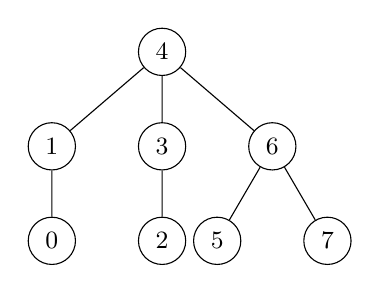
\begin{tikzpicture}[
  level distance=12mm, sibling distance=14mm,
  every node/.style={circle,draw,minimum size=6mm,inner sep=0pt,
    font=\small}
]
\node {4}
  child { node {1}
    child { node {0} }
  }
  child { node {3}
    child { node {2} }
  }
  child { node {6}
    child { node {5} }
    child { node {7} }
  };
\end{tikzpicture}
\end{center}

This tree is \emph{not} index-monotonic: node~7 has parent~6,
violating the condition $\text{label}(\text{parent}) >
\text{label}(\text{child})$ since $6 < 7$.

%%====================================================================
\subsection*{Index sets from Construction~A}

Applying the generic index-set computation:
\begin{center}
\begin{tabular}{@{}clll@{}}
\toprule
$j$ & $\Uset{j}$ & $\Rset{j}$ & $\Occ{j}$ \\
\midrule
0 & $\{1, 4\}$       & $\emptyset$     & $\{0\}$ \\
1 & $\{4\}$           & $\{0\}$         & $\{0, 1\}$ \\
2 & $\{3, 4\}$       & $\{1\}$         & $\{2\}$ \\
3 & $\{4\}$           & $\{1, 2\}$     & $\{2, 3\}$ \\
4 & $\emptyset$       & $\{1, 3\}$     & $\{0,1,2,3,4,5,6,7\}$ \\
5 & $\{6, 4\}$       & $\{1, 3\}$     & $\{5\}$ \\
6 & $\{4\}$           & $\{1, 3, 5\}$ & $\{5, 6, 7\}$ \\
7 & $\{6, 4\}$       & $\{1, 3, 5\}$ & $\{7\}$ \\
\bottomrule
\end{tabular}
\end{center}

%%====================================================================
\subsection*{Majorana operators (partial)}

From these index sets, the Majorana operators for modes 4 and~7 are:
\begin{align*}
  c_4 &= -Y_1 Y_3 X_4 Z_5 Z_6 Z_7, \\
  d_4 &= Y_1 Y_3 Y_4 Z_5 Z_6 Z_7, \\
  c_7 &= -Y_1 Y_3 Y_5 X_6 X_7, \\
  d_7 &= Y_1 Y_3 Y_5 X_6 Y_7.
\end{align*}
(Operators on unlisted qubits are identity.)

%%====================================================================
\subsection*{Failed anticommutator}

Computing $\acomm{\an{4}}{\ad{7}}$, where
$\an{4} = \frac{1}{2}(c_4 + i\,d_4)$ and
$\ad{7} = \frac{1}{2}(c_7 - i\,d_7)$:

\begin{align*}
  \acomm{\an{4}}{\ad{7}}
    &= \tfrac{1}{4}\bigl[
      \acomm{c_4}{c_7} + i\,\acomm{d_4}{c_7} \\
    &\quad\quad\;  - i\,\acomm{c_4}{d_7} + \acomm{d_4}{d_7}
    \bigr].
\end{align*}

For a valid encoding, this should vanish ($4 \neq 7$).  Instead:
\begin{align*}
  \acomm{c_4}{c_7} &= -2\,ZZZZZIZZ, \\
  \acomm{d_4}{d_7} &= +2\,ZZZZZIZZ, \\
  \acomm{c_4}{d_7} &= -2i\,ZZZZZIZZ, \\
  \acomm{d_4}{c_7} &= -2i\,ZZZZZIZZ.
\end{align*}

These do \emph{not} cancel in the linear combination:
\begin{equation*}
  \acomm{\an{4}}{\ad{7}} = (0.5i)\; ZZZZZIXY + (-0.5)\; ZZZZZIXX
    \neq 0.
\end{equation*}

%%====================================================================
\subsection*{Diagnosis}

The failure arises because nodes~6 and~7 share the parent--child
edge with $\text{label}(6) < \text{label}(7)$.  In the remainder-set
computation for $j = 7$:
\[
  \Rset{7} = \{v : v \text{ is a child of an ancestor of } 7,\;
    v < 7,\; v \notin \text{path}(7)\} = \{1, 3, 5\}.
\]
The $Z$-operators placed on qubits $\{1, 3, 5\}$ via the remainder
set of mode~7 overlap with $\Uset{4} = \emptyset$ and $\Rset{4} =
\{1, 3\}$, creating cross-mode interference in the anticommutator.
For a star tree, all remainder sets consist only of siblings, which
never overlap with update or occupation sets of other modes.

%%====================================================================
\subsection*{Verification by Construction~B}

Applying Construction~B (path-based encoding,
\cref{sec:tree-encoding}, \cref{sec:constructions}) to the \emph{same} balanced ternary tree
produces Majorana operators that satisfy \emph{all} $\binom{16}{2} =
120$ anticommutation relations exactly.  The tree topology is not the
problem; the index-set derivation method is.


\section{Algebraic Data Types}
\label{app:datatypes}
\input{drafts/appendix-c-datatypes}

\end{document}
